\begin{savequote}[8cm]
Simplicity is prerequisite for reliability.
  \qauthor{--- Edsger W. Dijkstra}
\end{savequote}

\chapter{An introduction to high-level modular assembly}

\minitoc

Already from the start, the field of structural DNA nanotechnology has been interested in modular assemblies, although initially in the form of infinite chrystal structures. Prof. Ned Seeman was inspired to pioneer the field after seeing the woodcut \emph{Depth} by M.C. Escher \cite{seeman_2016}, where fish are depicted organised into a neat chrystalline structure.

But components that self-assemble into chrystals can also be made to assemble into bounded structures, given that a way can be found to make them self-limiting. This chapter will provide an overview on the background of self-assembled multi-component structures, starting with experimental results of ever-increasing size and followed by a selection of theoretical models.

\section{Experimental applications} \label{sec:experimental_appl}
From small tiles made from a handful of strands to megadalton-scale structures made from multiple origamis, modular assembly has seen a lot of experimental research. This section will detail some results of particular interest to the polycube model presented in Chapter \ref{ch:3-polycubes}.

\subsection{DNA tiles and bricks}
% Tiles: https://www.nature.com/articles/28998

\begin{figure}[h]
  \centering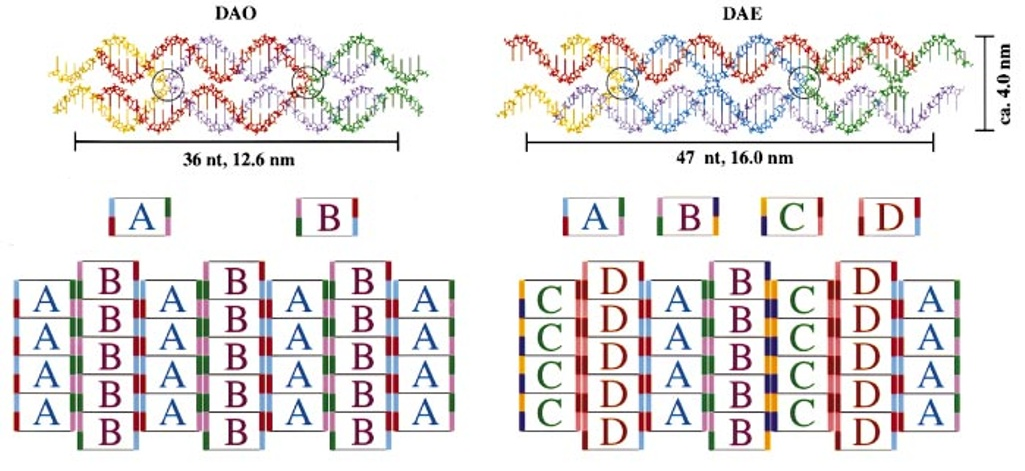
\includegraphics[width=\textwidth]{figures/dna_tiles.png}
  \caption{DX tiles forming 2D lattices, adapted from \cite{winfree1998design}. a) Lattices made from two units and four units respectively. b) Examples of DAO and DAE tile designs.}
  \label{fig:dna_tiles}
\end{figure}

% Bricks: https://www.nature.com/articles/nature24648

\begin{figure}[h]
  \centering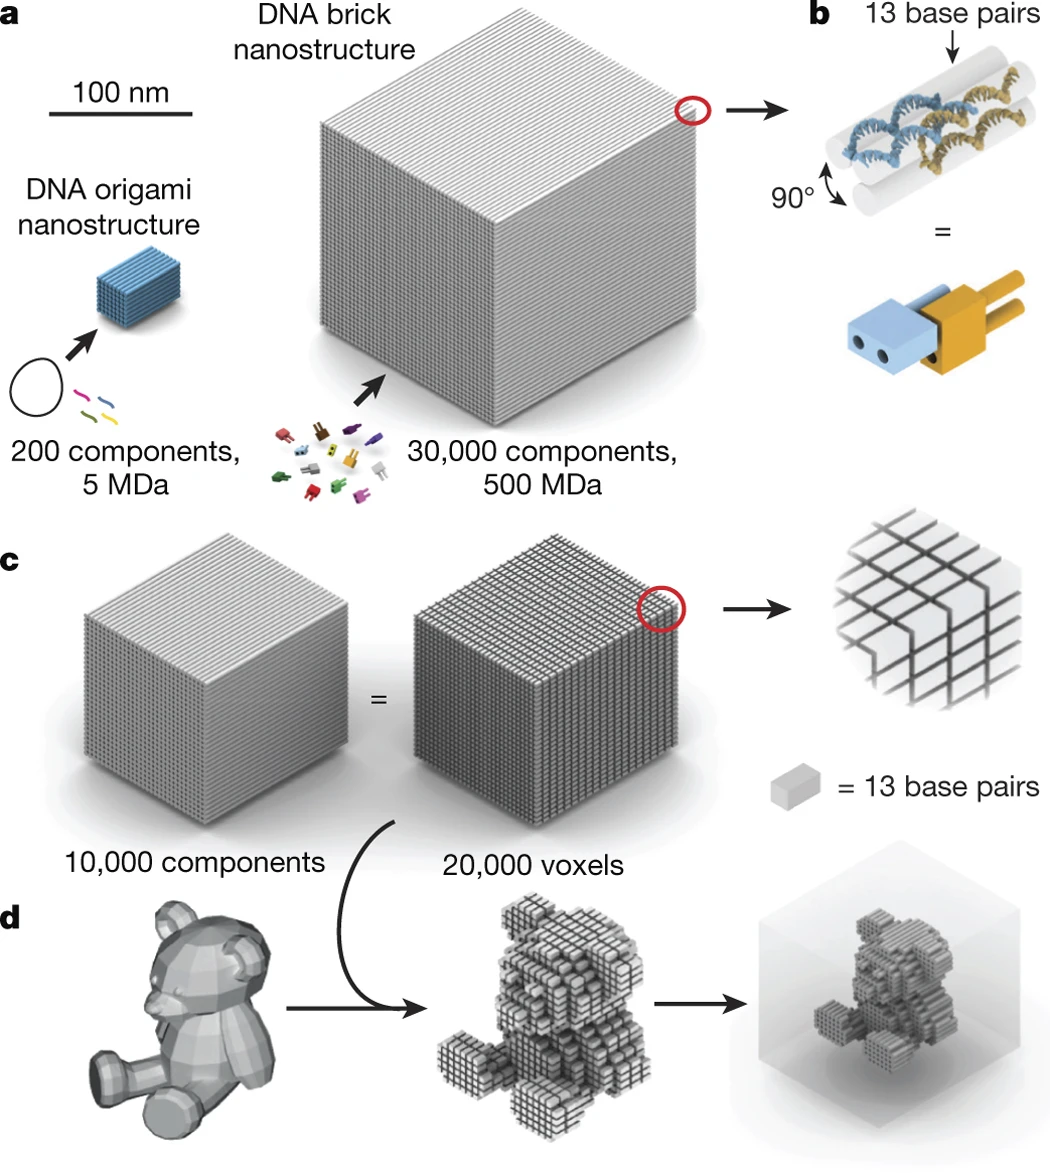
\includegraphics[width=0.6\textwidth]{figures/dna_bricks.png}
  \caption{3D bricks from \cite{ong2017programmable}}
  \label{fig:dna_tiles}
\end{figure}

\subsection{RNA tiles}
%https://www.science.org/doi/abs/10.1126/science.1253920 
In 2014, Cody Geary published a method of folding RNA tiles co-transcriptionally \cite{geary2014single}. The design used a set of tertiary RNA motifs, such as kissing hairpins and double crossovers, to fold the RNA strand into the desired tile structure. The tiles then assembled connected by complementary 120-degree kissing loop interactions. The design method was later described in depth in the \emph{Methods in Molecular Biology} book series \cite{sparvath2017computer}.

\begin{figure}[h]
  \centering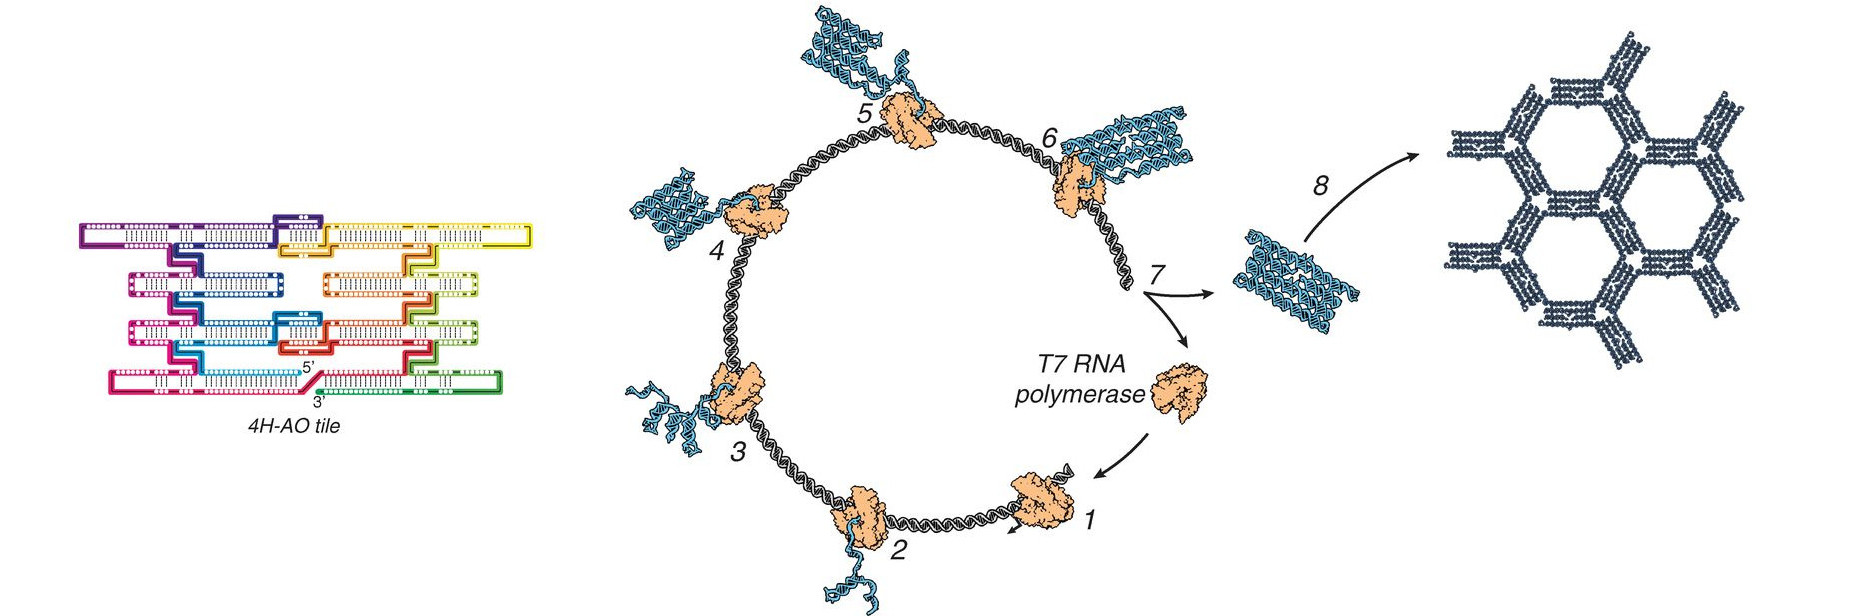
\includegraphics[width=\textwidth]{figures/rna_tiles.jpeg}
  \caption{2D RNA tiles from \cite{geary2014single}}
  \label{fig:rna_tiles}
\end{figure}

\subsection{DNA origami arrays}\label{sec:origamiArrays}
% https://www.nature.com/articles/nature24655

In 2017, Tikhomirov, et al.\cite{tikhomirov2017fractal} demonstrated two-dimensional patterns assembled on the micrometre-scale using square origami tiles connecting through their complementary edges. helices

\begin{figure}[h]
  \centering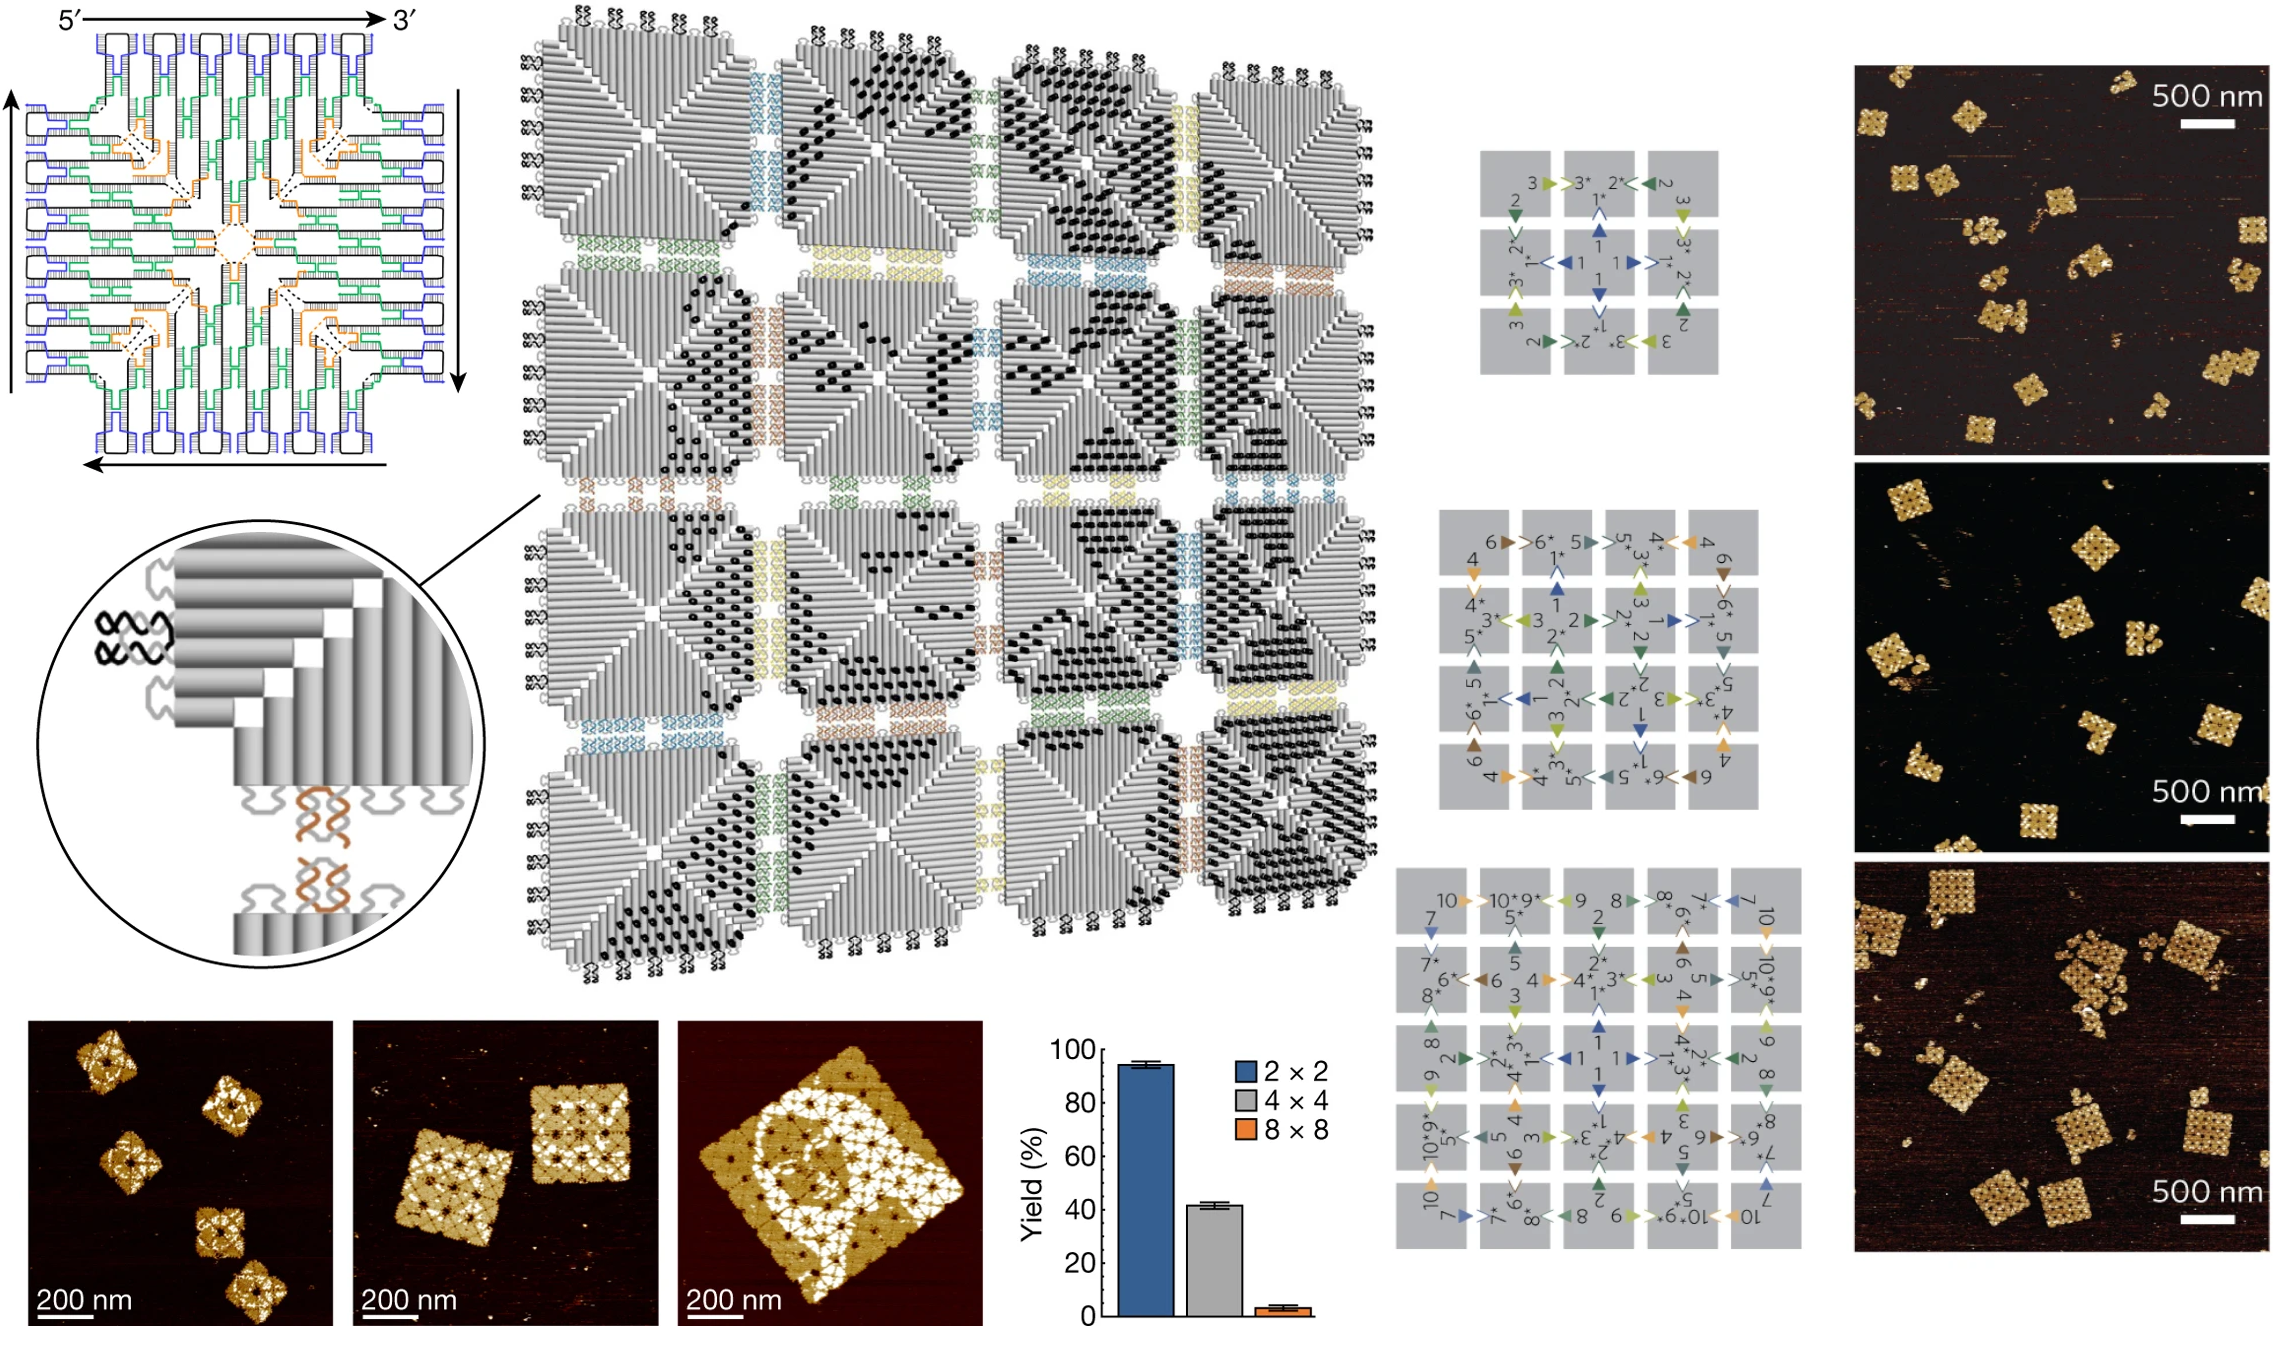
\includegraphics[width=0.6\textwidth]{figures/monalisa_tiles.png}
  \caption{Adapted from \cite{tikhomirov2017fractal}}
\end{figure}

\subsection{Shape-complementary origami}
% 2D https://www.nature.com/articles/nchem.1070
% 3D https://science.sciencemag.org/content/347/6229/1446.abstract

% Huge https://www.nature.com/articles/s41563-021-01020-4

Also in 2017, Wagenbauer, et al. \cite{wagenbauer2017gigadalton} used shape-complementarity to assemble origami tiles into three-dimensional polyhedral shapes up to 450 nanometers in diameter.

\begin{figure}[h]
  \centering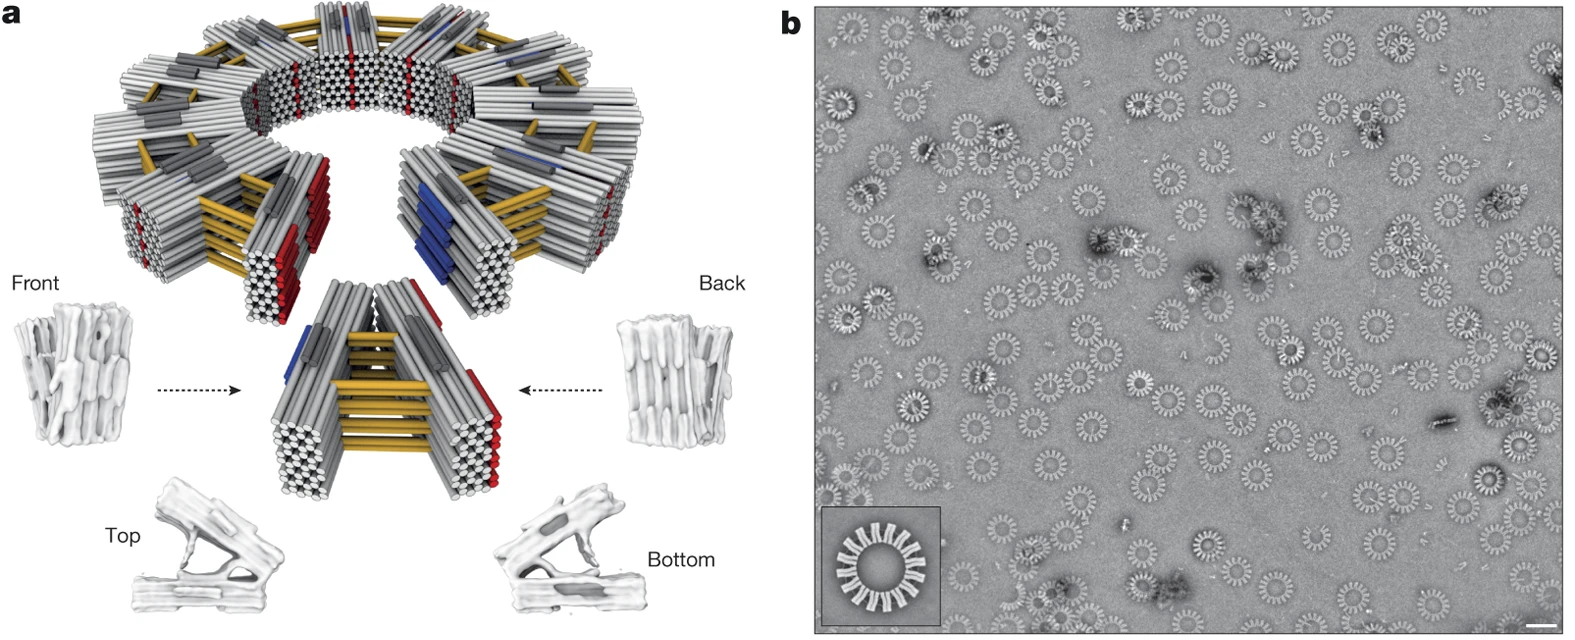
\includegraphics[width=0.6\textwidth]{figures/dietz_ring.png}
  \caption{Adapted from \cite{wagenbauer2017gigadalton}}
\end{figure}

\cite{sigl2021programmable}


\subsection{DNA origami nanochambers}
% https://pubs.acs.org/doi/full/10.1021/jacs.0c07263

\begin{figure}[h]
  \centering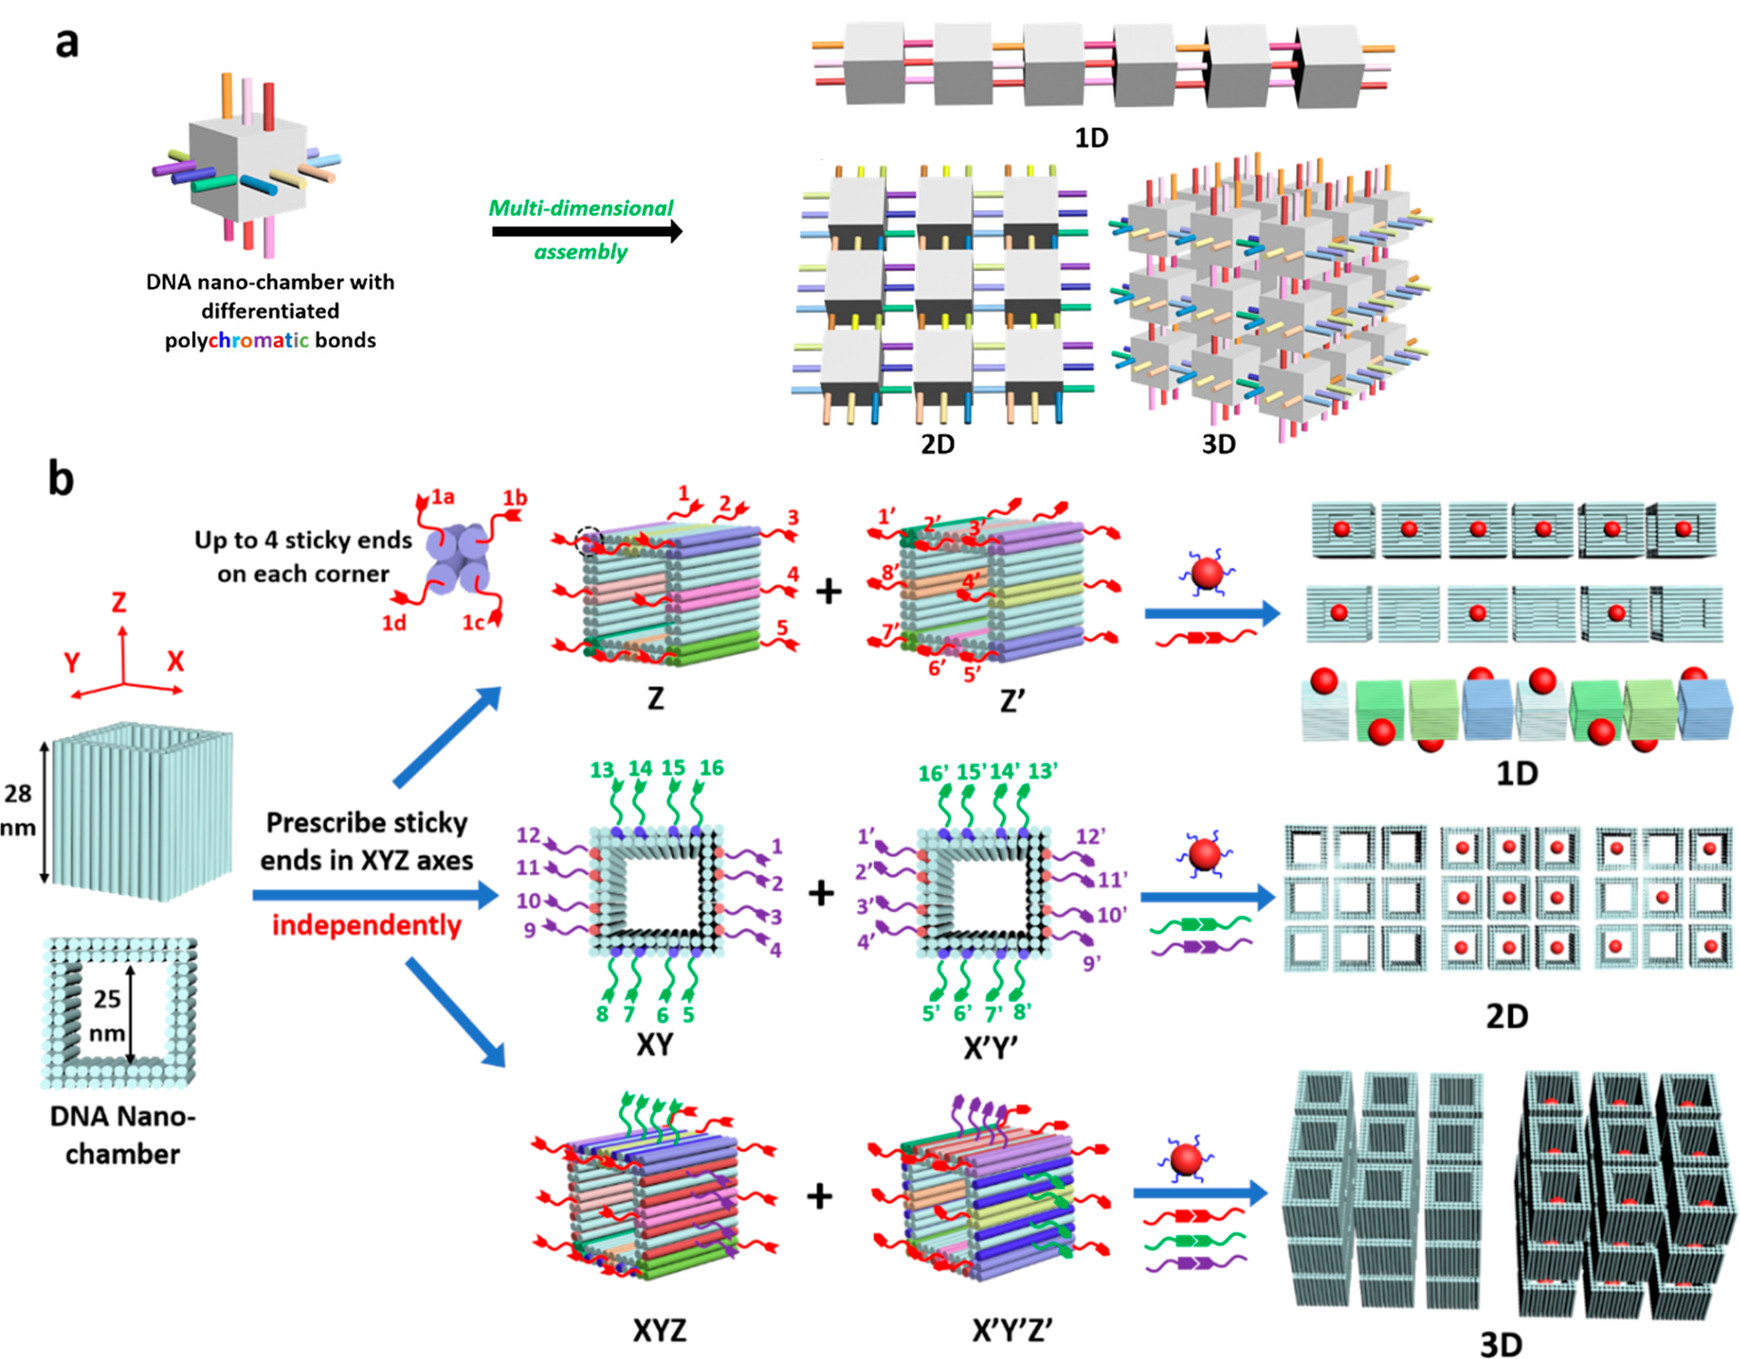
\includegraphics[width=\textwidth]{figures/nanochambers2.jpeg}
  \caption{DNA nanochambers, adapted from \cite{nano-chambers_lin2020}}
\end{figure}

\subsection{Octahedral DNA origami frames}
% https://onlinelibrary.wiley.com/doi/abs/10.1002/anie.201913958

\begin{figure}[h]
  \centering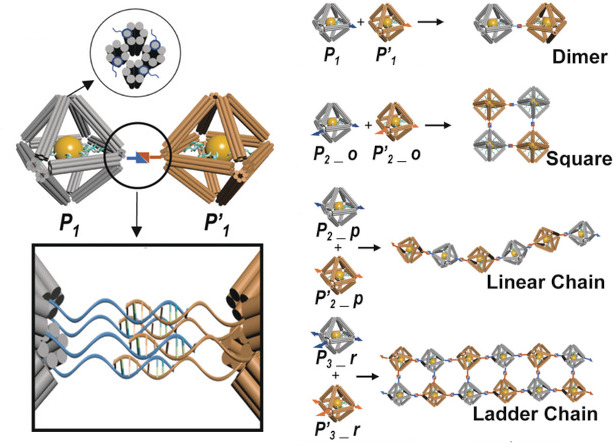
\includegraphics[width=\textwidth]{figures/tian.jpg}
  \caption{Octahedral DNA origami frames, adapted from \cite{tian_octahedra2020}}
\end{figure}




\section{Modular assembly models}
It would be computationally unreasonable to simulate module assemblhelicesy at the level of individual nucleotides. A better approach is instead to use an abstract model to predict the assembly process with the modules treated as rigid bodies. This section will present earlier such models as a background to my own model described in Chapter \ref{ch:3-polycubes}.

\subsection{Wang tiles}
Introduced by Hao Wang in 1961 \cite{wang1961proving}, so called \emph{Wang tiles} are 

\begin{figure}[h]
  \centering\includesvg[width=0.6\textwidth]{figures/Wang_11_tiles.svg}
  \caption{Wang tiles}
\end{figure}

\subsection{The algorithmic tile assembly model}

% David Doty overview: https://cacm.acm.org/magazines/2012/12/157881-theory-of-algorithmic-self-assembly/fulltext

% Molecular algorithms https://www.nature.com/articles/s41586-019-1014-9

In his 1998 thesis Erik Winfree showed the usage of the double-crossover (DX) motif to create regular arrays \cite{winfree1998design}. These tiles behave like Wang tiles\cite{wang1961proving} and do not allow rotations or reflections. Winfree also investigated the possibility of using such tiles for computation \cite{winfree1998algorithmic}.
% DX array https://www.nature.com/articles/28998

Co-operative binding

\begin{figure}[h]
  \centering\includesvg[width=\textwidth]{figures/atam.svg}
  \caption{Algorithmic self-assembly model}
\end{figure}

\subsection{The polyomino model}\label{sec:polyomino}

The main inspiration for the polycube model presented in Chapter \ref{ch:3-polycubes} is the polyomino model \cite{ahnert2010self}\cite{johnston2011evolutionary}. The main difference to aTAM is that polyomino tiles are allowed to rotate. They also have a constant binding strength (in other words, it is a temperature-1 model).

%, studying the self-assembly, modularity and evolutionary dynamics of \emph{polyominoes}.

Polyominoes are abstract structures composed of one or more squares, connected by their edges. The polyomino assembly model developed is similar in assembly to the later experimental micro-meter scale tile designs by Tikhomirov \cite{tikhomirov2017fractal} described in Section \ref{sec:origamiArrays}. Compared to Wang tiles\cite{wang1961proving}, the edge binding does not need to be between edges of the same colour, but can be specified by a more complex interaction matrix. Furthermore, the tiles can be rotated to bind, creating further possibilities for symmetries.

\begin{figure}[h]
    \centering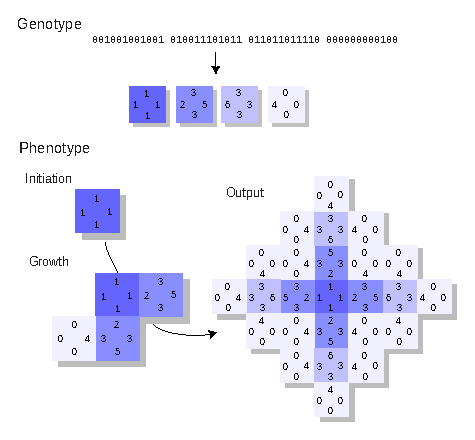
\includegraphics[width=0.6\textwidth]{figures/polyominoes.eps}
    \caption{Illustration of the polyomino assembly model used by Johnston. A \emph{genotype}, in the form of a ruleset of possible tiles, encodes for a polyomino \emph{phenotype}, grown stochastically from an initial seed tile. Image adapted from \cite{johnston2011evolutionary}.}
    \label{fig:polyominoes}
\end{figure}

I aim to build on Johnston's work on polyominoes to explore the properties of such self-assembling systems in three dimensions; the self-assembly of \emph{polycubes}. With such a model in place, it should be possible to design, through shape complementary in DNA origami \cite{wagenbauer2017gigadalton}, kissing interactions in RNA origami \cite{geary2014single}, or other methods, robotic modules with the interfaces necessary to assemble into the desired polycube shape. My current progress within this project is covered in Chapter \ref{ch:3-polycubes}.

\subsection{Patchy particles}

\section{Algorithmic Information Theory and input-output maps}
% https://www.ox.ac.uk/news/science-blog/%E2%80%98simplicity-bias%E2%80%99-science

% https://www.nature.com/articles/s41467-018-03101-6

% https://solo.bodleian.ox.ac.uk/permalink/f/89vilt/oxfaleph022417805

%Some things, whether in the form of a shape, a song, or a binary string, require less information to describe than others.

If you have a monkey pressing random keys on a typewriter, you would expect it to produce every string of length \(N\) with equal probability (assuming the keystrokes were indeed truly random). With \(k\) keys on the keyboard, the probability for any string of length \(N\) is then \(k^{-N}\). For example, the title of this thesis, while unlikely to appear randomly, would be equally as probable as any other 50-character string, see the three example strings below:
\begin{lstlisting}[numbers=left]
  DESIGN AND MODULAR SELF-ASSEMBLY OF NANOSTRUCTURES
  SHWDRVWKFORWJDOEXOZLSBNREKC Z  VSDJJF  ROKFYRVMIUI
  AAAAAAAAAAAAAAAAAAAAAAAAAAAAAAAAAAAAAAAAAAAAAAAAAA
\end{lstlisting}

However, some strings can have a description shorter than a full listing of the letters it contains. For example, string number three above could be described simply as ``Print \texttt{A}, 50 times'', or if we use the C programming language:

\begin{lstlisting}[language=c]
for(int i=50; i--;) printf("A");
\end{lstlisting}

There are also a number of possible valid variations of the code avove, with different variable names and coding conventions, all producing the same output. In other words, not only is the description shorter than writing out the full string, but there are also multiple inputs that map to the same output, increasing the probability further.

The concept of using the shortest possible computer program that can describe an object (for example, a binary string) to determine its complexity is central within the field of Algorithmic Information Theory (AIT) and is called Kolmogorov complexity (or Solomonoff–Kolmogorov–Chaitin to give full credit) \cite{LiMing2019AitK}. More specifically, the Kolmogorov complexity \(K(x)\) of an output \(x\) is the length of the shortest program that generates \(x\) on a Universal Turing Machine (UTM).

AIT includes the \emph{coding theorem}, introducing lower and upper bounds for the probability \(P(x)\) of generating a binary string \(x\) as \(2^{-K(x)} \le P(x) \le 2^{-K(x) + \mathcal{O} (1)}\). In other words, low-complexity outputs are exponentially more likely to generated by random input compared to high-complexity outputs. This could be compared to how, intuitively, there are likely more programs generating the ``simple'' string number 3 above compared to the randomly generated number 2.

However, finding the shortest program for an output is far from trivial (in general, it is in fact \emph{uncomputable}, due to the \emph{halting problem}). Fortunately, Dingle at al \cite{dingle2018input} were able to derive an upper bound to the probability using a computable approximation \(\widetilde{K}(x)\) of the Komologrov complexity:

\[
  P(x) \lesssim 2^{-a\widetilde{K}(x) -b}
\]

where \(a\) and \(b\) are constants that depend on the input-output map used (but are independent of \(x\)).


